\documentclass{article}

\usepackage[utf8]{inputenc}
\usepackage[brazil]{babel}

\title{Exercício 3: Aproximação Polinomial}
\author{Rúbia Reis Guerra \\ 2013031143}

\usepackage{Sweave}
\begin{document}
\Sconcordance{concordance:aprox.tex:aprox.Rnw:%
1 8 1 1 0 7 1 1 2 1 0 1 1 1 2 1 0 1 1 1 2 1 1 1 2 1 1 1 2 1 1 1 2 5 0 2 %
2 1 0 4 1 1 2 1 1 1 2 5 0 2 2 1 0 4 1 1 2 1 1 1 2 5 0 2 2 1 0 4 1 1 2 1 %
1 1 2 5 0 2 2 1 0 4 1 1 2 1 1 1 2 5 0 2 2 1 0 4 1 1 2 1 1 1 2 5 0 2 2 1 %
0 4 1 1 2 1 1 1 2 5 0 2 2 1 0 4 1 1 2 1 1 1 2 5 0 2 2 1 0 4 1 1 2 1 1 1 %
2 5 0 1 2 2 1 1 2 1 0 1 1 1 2 1 0 1 1 1 2 1 1 1 2 1 1 1 2 1 1 1 2 5 0 2 %
2 1 0 4 1 1 2 1 1 1 2 5 0 1 2 1 1 1 2 1 0 4 1 1 2 1 1 1 2 5 0 1 2 1 1 1 %
2 1 0 4 1 1 2 1 1 1 2 5 0 2 2 1 0 4 1 1 2 1 1 1 2 5 0 2 2 1 0 4 1 1 2 1 %
1 1 2 5 0 2 2 1 0 4 1 1 2 1 1 1 2 5 0 2 2 1 0 4 1 1 2 1 1 1 2 5 0 2 2 1 %
0 4 1 1 2 1 1 1 2 5 0 1 2 2 1}

\maketitle

\section{Introdução}
Nesta atividade, foi implementada a aproximação polinomial de uma função geradora $f_{g}(x)$. Em seguida, a partir da modificação do grau do polinômio $p(x)$, foram observados os fenômenos de \textit{underfitting} e \textit{overfitting} nos modelos resultantes.

\section{N = 10}
\begin{Schunk}
\begin{Sinput}
> rm(list=ls())
> library('corpcor')
> ######################
> N <- 10
> cores <- rainbow(8)
> X <- runif(n = N, min=-15, max=10)
> Y <- (0.5*(X^2)+3*X+10) + rnorm(length(X), 0, 4)
> xgrid <- seq(-15, 10, 0.1)
> ygrid <- (0.5*(xgrid^2)+3*xgrid+10)
> plot(X, Y, type='p', xlim=c(-15,10), ylim=c(0,120), xlab='', ylab='')
> par(new=T)
> plot(xgrid, ygrid, type='l', xlim=c(-15,10), ylim=c(0,120), 
+      col='black', xlab='', ylab='', sub = 'Função geradora, 10 amostras')
\end{Sinput}
\end{Schunk}
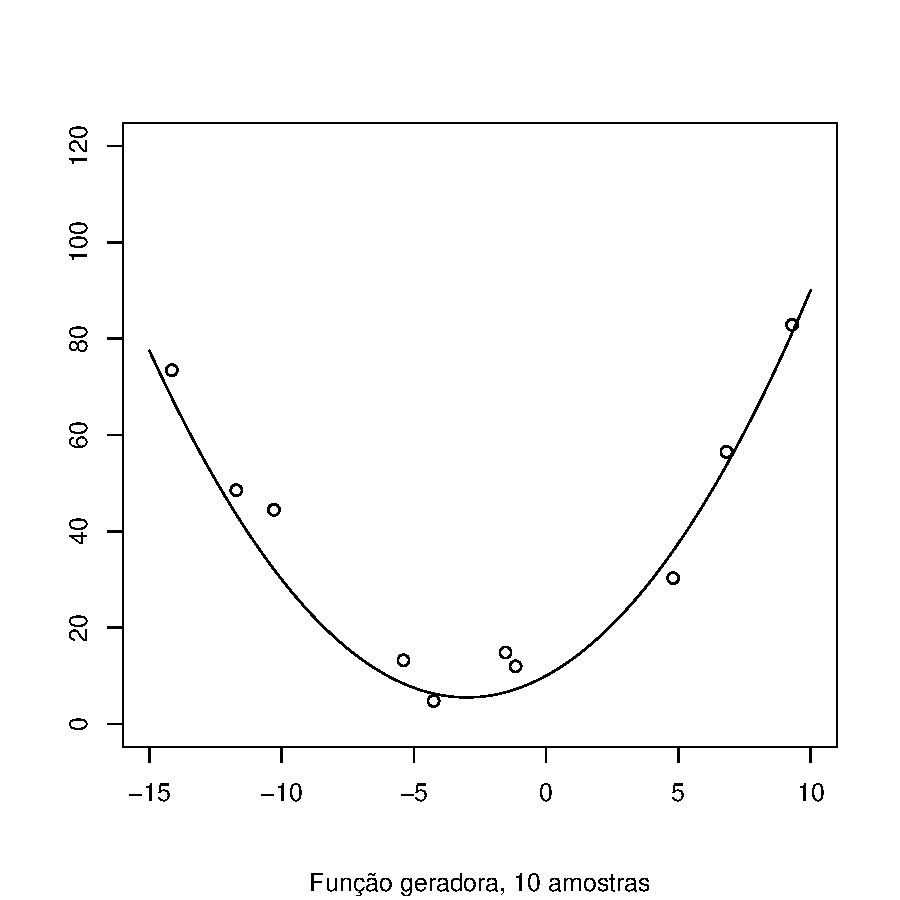
\includegraphics{aprox-001}
\subsection{p = 1}
\begin{Schunk}
\begin{Sinput}
> H <- cbind(X, 1)
> w <- pseudoinverse(H) %*% Y
> Hgrid <- cbind(xgrid, 1)
> yhat <- H %*% w
> yhatgrid <- Hgrid %*% w
> plot(X, Y, type='p', xlim=c(-15,10), ylim=c(0,120), xlab='', ylab='')
> par(new=T)
> plot(xgrid, yhatgrid, type='l', xlim=c(-15,10), ylim=c(0,120), 
+      col=cores[1], xlab='x', ylab='y', sub='10 amostras, p = 1, underfitting')
\end{Sinput}
\end{Schunk}
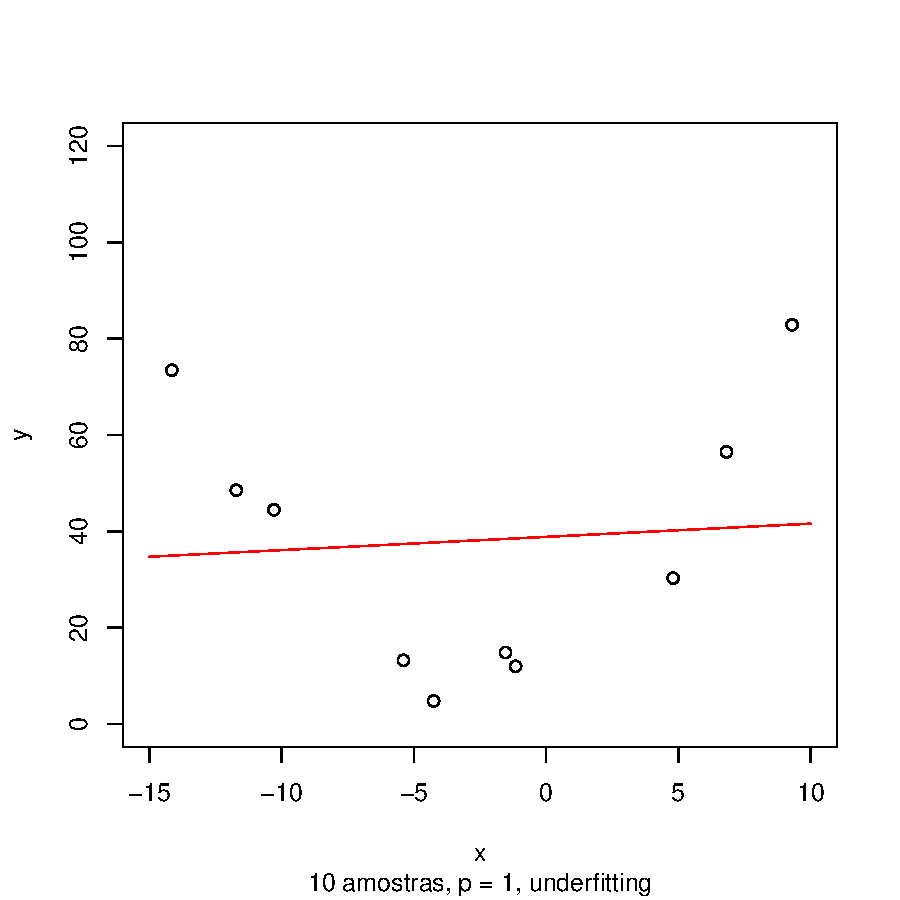
\includegraphics{aprox-002}
\subsection{p = 2}
\begin{Schunk}
\begin{Sinput}
> H <- cbind(X^2, X, 1)
> w <- pseudoinverse(H) %*% Y
> Hgrid <- cbind(xgrid^2, xgrid, 1)
> yhat <- H %*% w
> yhatgrid <- Hgrid %*% w
> plot(X, Y, type='p', xlim=c(-15,10), ylim=c(0,120), xlab='', ylab='')
> par(new=T)
> plot(xgrid, yhatgrid, type='l', xlim=c(-15,10), ylim=c(0,120), 
+      col=cores[2], xlab='x', ylab='y', sub='10 amostras, p = 2, modelo balanceado')
\end{Sinput}
\end{Schunk}
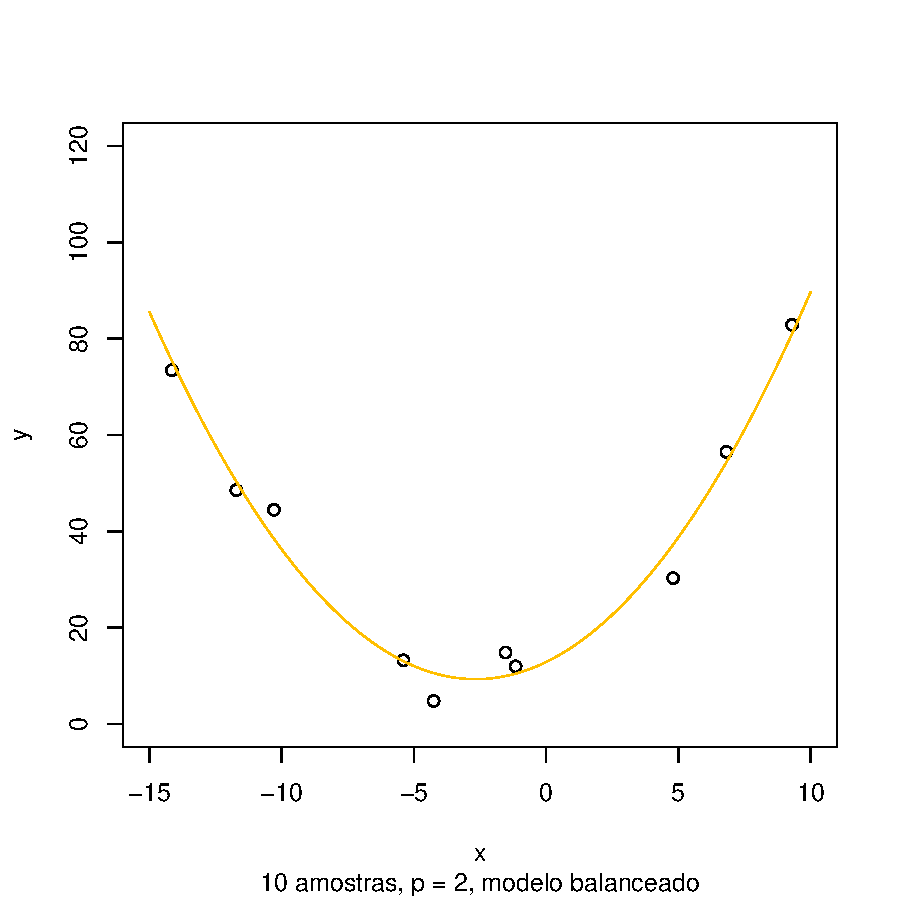
\includegraphics{aprox-003}
\subsection{p = 3}
\begin{Schunk}
\begin{Sinput}
> H <- cbind(X^3, X^2, X, 1)
> w <- pseudoinverse(H) %*% Y
> Hgrid <- cbind(xgrid^3, xgrid^2, xgrid, 1)
> yhat <- H %*% w
> yhatgrid <- Hgrid %*% w
> plot(X, Y, type='p', xlim=c(-15,10), ylim=c(0,120), xlab='', ylab='')
> par(new=T)
> plot(xgrid, yhatgrid, type='l', xlim=c(-15,10), ylim=c(0,120),
+      col=cores[3], xlab='x', ylab='y', sub='10 amostras, p = 3, modelo balanceado')
\end{Sinput}
\end{Schunk}
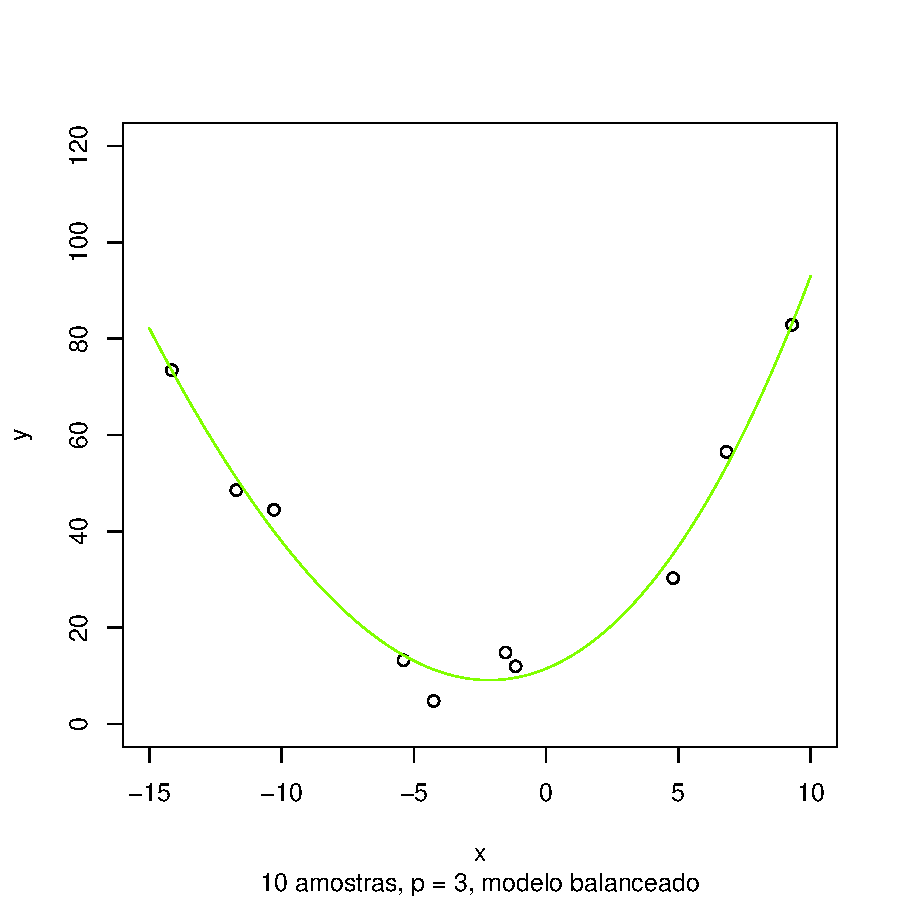
\includegraphics{aprox-004}
\subsection{p = 4}
\begin{Schunk}
\begin{Sinput}
> H <- cbind(X^4, X^3, X^2, X, 1)
> w <- pseudoinverse(H) %*% Y
> Hgrid <- cbind(xgrid^4, xgrid^3, xgrid^2, xgrid, 1)
> yhat <- H %*% w
> yhatgrid <- Hgrid %*% w
> plot(X, Y, type='p', xlim=c(-15,10), ylim=c(0,120), xlab='', ylab='')
> par(new=T)
> plot(xgrid, yhatgrid, type='l', xlim=c(-15,10), ylim=c(0,120),
+      col=cores[4], xlab='x', ylab='y', sub='10 amostras, p = 4, modelo balanceado')
\end{Sinput}
\end{Schunk}
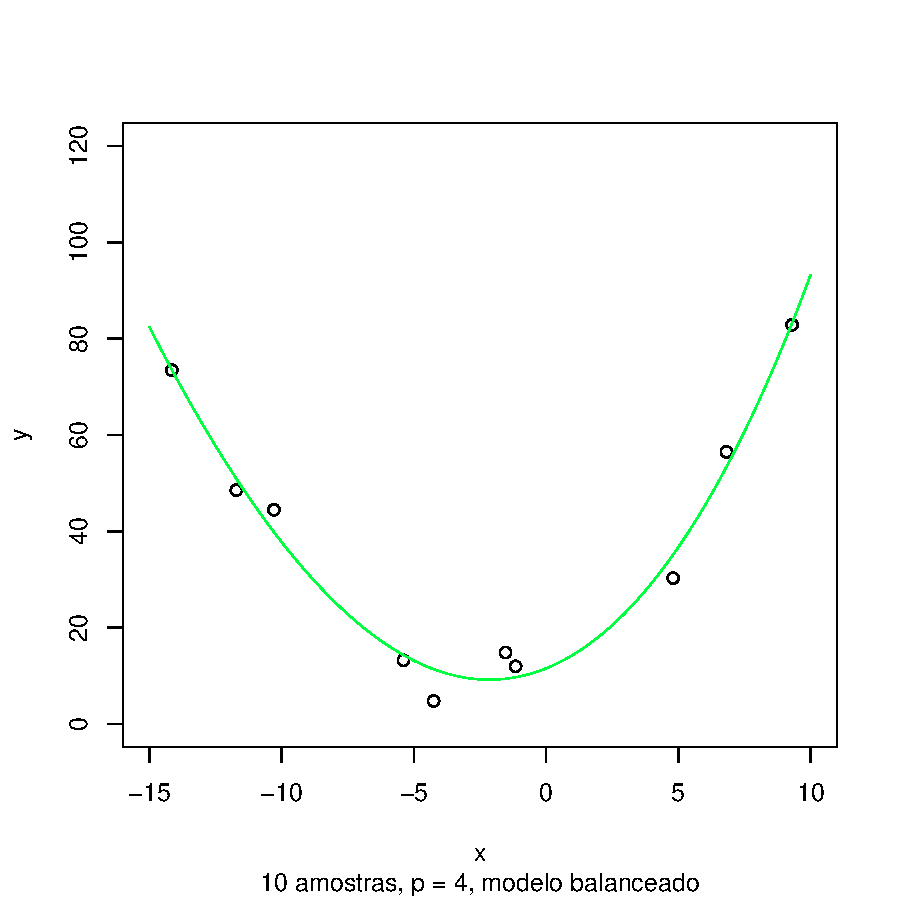
\includegraphics{aprox-005}
\subsection{p = 5}
\begin{Schunk}
\begin{Sinput}
> H <- cbind(X^5, X^4, X^3, X^2, X, 1)
> w <- pseudoinverse(H) %*% Y
> Hgrid <- cbind(xgrid^5, xgrid^4, xgrid^3, xgrid^2, xgrid, 1)
> yhat <- H %*% w
> yhatgrid <- Hgrid %*% w
> plot(X, Y, type='p', xlim=c(-15,10), ylim=c(0,120), xlab='', ylab='')
> par(new=T)
> plot(xgrid, yhatgrid, type='l', xlim=c(-15,10), ylim=c(0,120),
+      col=cores[5], xlab='x', ylab='y', sub='10 amostras, p = 5, overfitting')
\end{Sinput}
\end{Schunk}
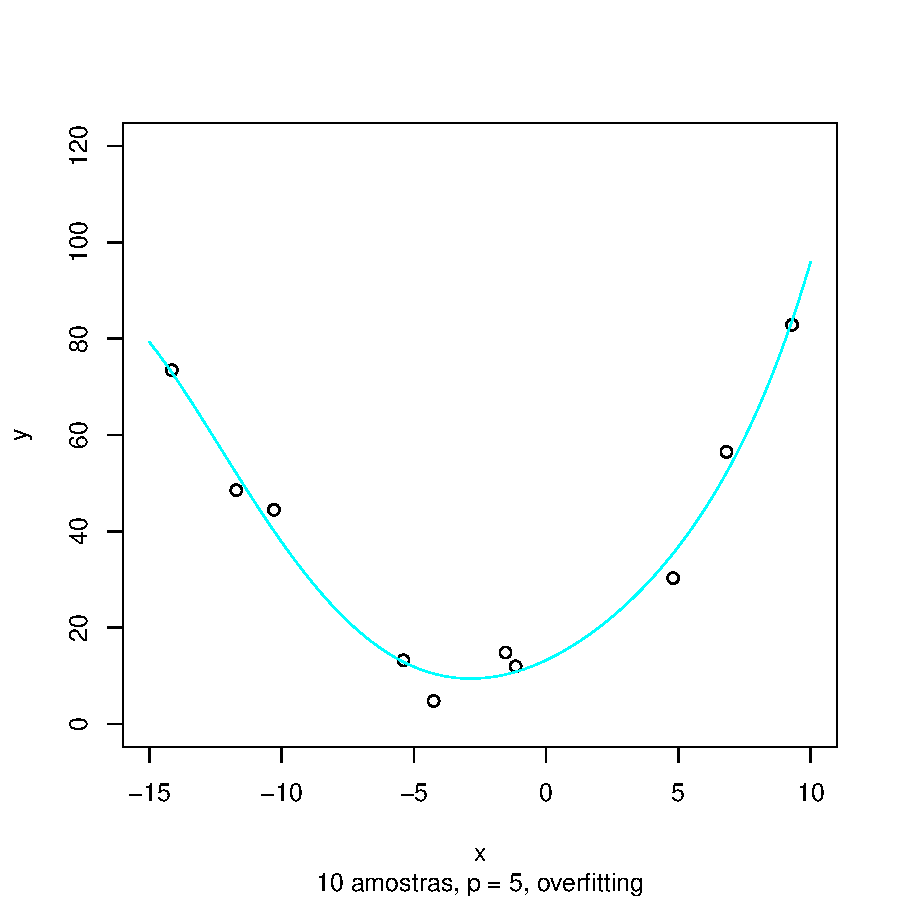
\includegraphics{aprox-006}
\subsection{p = 6}
\begin{Schunk}
\begin{Sinput}
> H <- cbind(X^6, X^5, X^4, X^3, X^2, X, 1)
> w <- pseudoinverse(H) %*% Y
> Hgrid <- cbind(xgrid^6, xgrid^5, xgrid^4, xgrid^3, xgrid^2, xgrid, 1)
> yhat <- H %*% w
> yhatgrid <- Hgrid %*% w
> plot(X, Y, type='p', xlim=c(-15,10), ylim=c(0,120), xlab='', ylab='')
> par(new=T)
> plot(xgrid, yhatgrid, type='l', xlim=c(-15,10), ylim=c(0,120),
+      col=cores[6], xlab='x', ylab='y', sub='10 amostras, p = 6, overfitting')
\end{Sinput}
\end{Schunk}
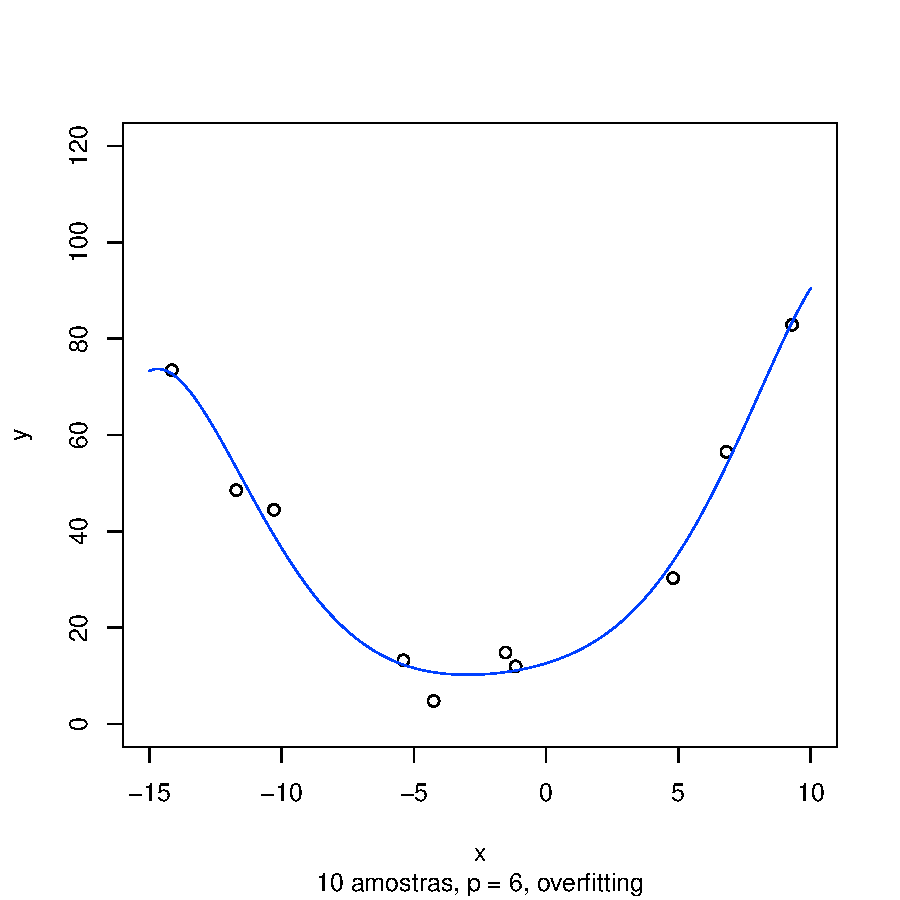
\includegraphics{aprox-007}
\subsection{p = 7}
\begin{Schunk}
\begin{Sinput}
> H <- cbind(X^7, X^6, X^5, X^4, X^3, X^2, X, 1)
> w <- pseudoinverse(H) %*% Y
> Hgrid <- cbind(xgrid^7, xgrid^6, xgrid^5, xgrid^4, xgrid^3, xgrid^2, xgrid, 1)
> yhat <- H %*% w
> yhatgrid <- Hgrid %*% w
> plot(X, Y, type='p', xlim=c(-15,10), ylim=c(0,120), xlab='', ylab='')
> par(new=T)
> plot(xgrid, yhatgrid, type='l', xlim=c(-15,10), ylim=c(0,120),
+      col=cores[7], xlab='x', ylab='y', sub='10 amostras, p = 7, overfitting')
\end{Sinput}
\end{Schunk}
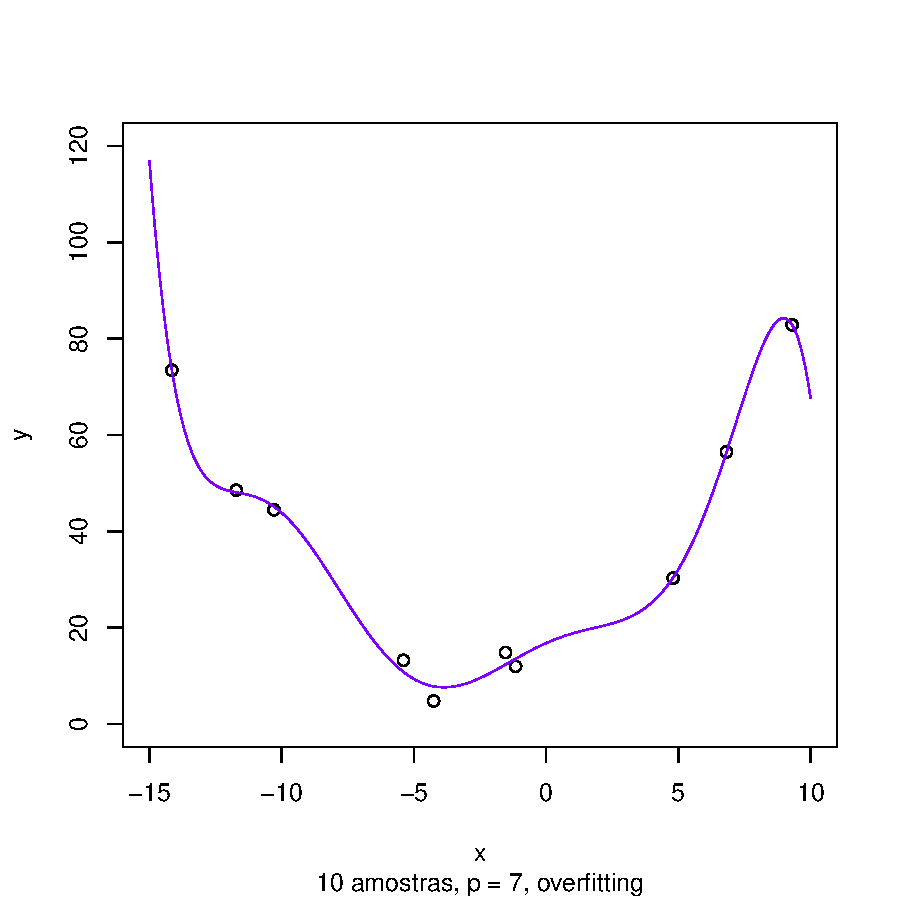
\includegraphics{aprox-008}
\subsection{p = 8}
\begin{Schunk}
\begin{Sinput}
> H <- cbind(X^8, X^7, X^6, X^5, X^4, X^3, X^2, X, 1)
> w <- pseudoinverse(H) %*% Y
> Hgrid <- cbind(xgrid^8, xgrid^7, xgrid^6, xgrid^5, xgrid^4, xgrid^3, xgrid^2, xgrid, 1)
> yhat <- H %*% w
> yhatgrid <- Hgrid %*% w
> plot(X, Y, type='p', xlim=c(-15,10), ylim=c(0,120), xlab='', ylab='')
> par(new=T)
> plot(xgrid, yhatgrid, type='l', xlim=c(-15,10), ylim=c(0,120),
+      col=cores[8], xlab='x', ylab='y', sub='10 amostras, p = 8, overfitting')
\end{Sinput}
\end{Schunk}
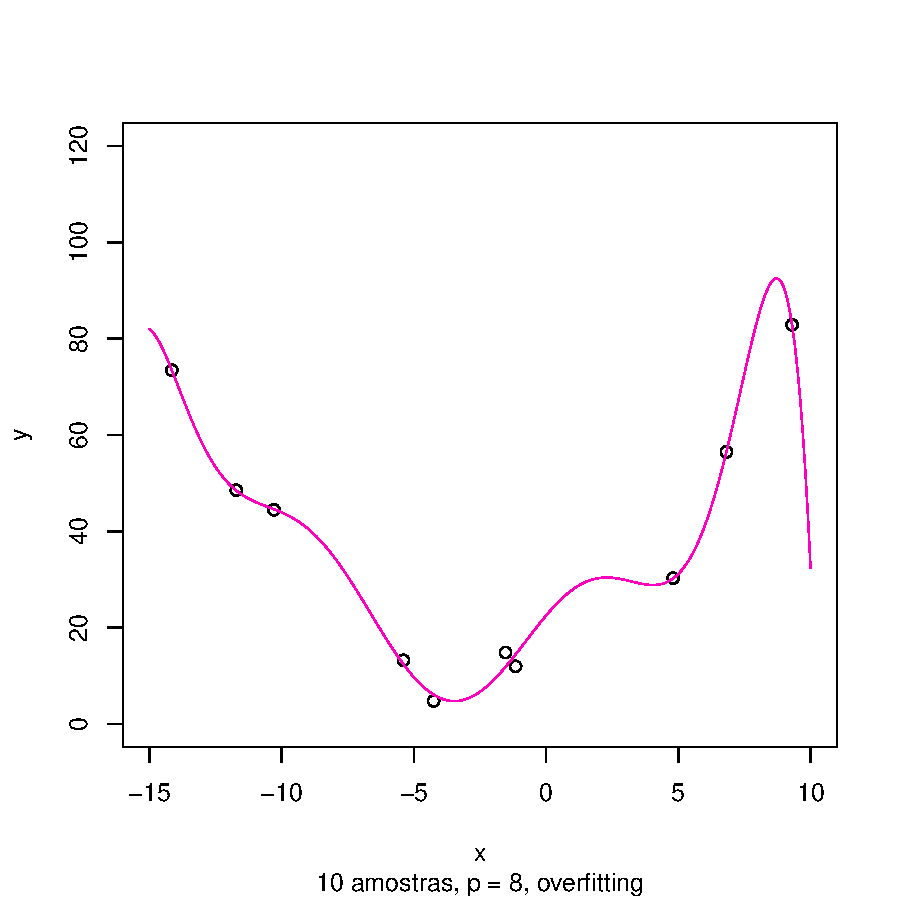
\includegraphics{aprox-009}

\section{N = 100}
Com um maior número de amostras, o modelo é menos sensível a flutuações nos dados (menor variância) e, como consequência, é menos propenso a overfitting.
\begin{Schunk}
\begin{Sinput}
> rm(list=ls())
> library('corpcor')
> ######################
> N <- 100
> cores <- rainbow(8)
> X <- runif(n = N, min=-15, max=10)
> Y <- (0.5*(X^2)+3*X+10) + rnorm(length(X), 0, 4)
> xgrid <- seq(-15, 10, 0.1)
> ygrid <- (0.5*(xgrid^2)+3*xgrid+10)
> plot(X, Y, type='p', xlim=c(-15,10), ylim=c(0,120), xlab='', ylab='')
> par(new=T)
> plot(xgrid, ygrid, type='l', xlim=c(-15,10), ylim=c(0,120), 
+      col='black', xlab='', ylab='', sub = 'Função geradora, 100 amostras')
\end{Sinput}
\end{Schunk}
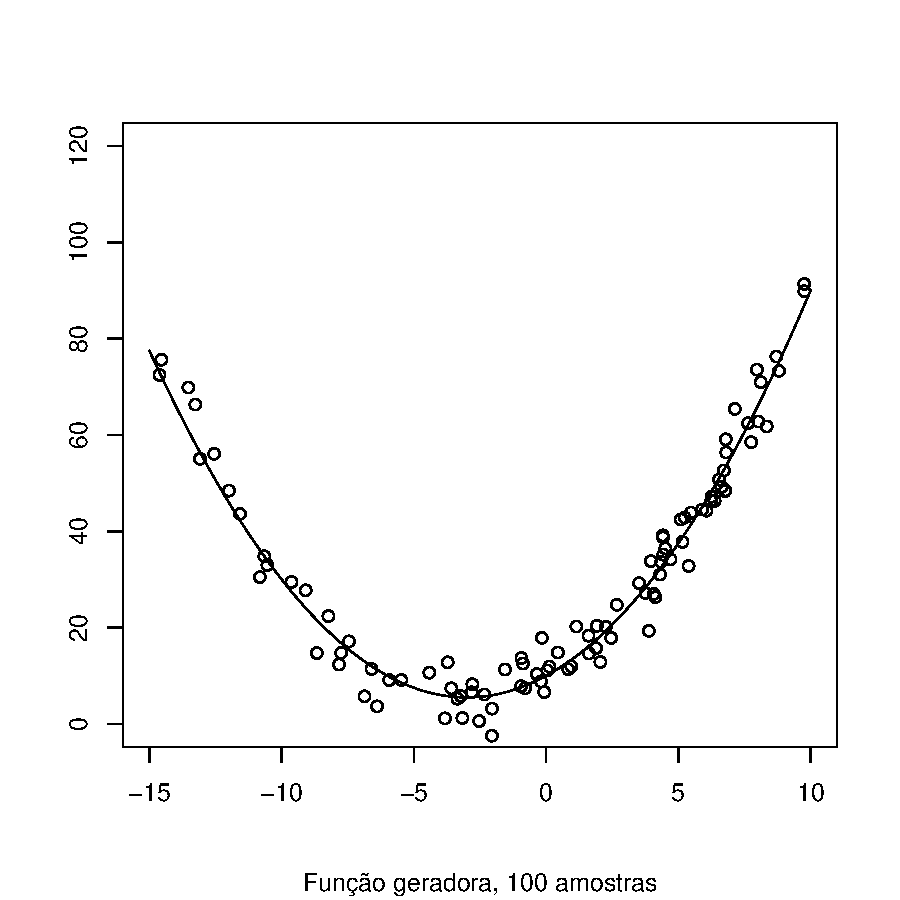
\includegraphics{aprox-010}
\subsection{p = 1}
\begin{Schunk}
\begin{Sinput}
> H <- cbind(X, 1)
> w <- pseudoinverse(H) %*% Y
> Hgrid <- cbind(xgrid, 1)
> yhat <- H %*% w
> yhatgrid <- Hgrid %*% w
> plot(X, Y, type='p', xlim=c(-15,10), ylim=c(0,120), xlab='', ylab='')
> par(new=T)
> plot(xgrid, yhatgrid, type='l', xlim=c(-15,10), ylim=c(0,120), 
+      col=cores[1], xlab='x', ylab='y', sub='100 amostras, p = 1, underfitting')
\end{Sinput}
\end{Schunk}
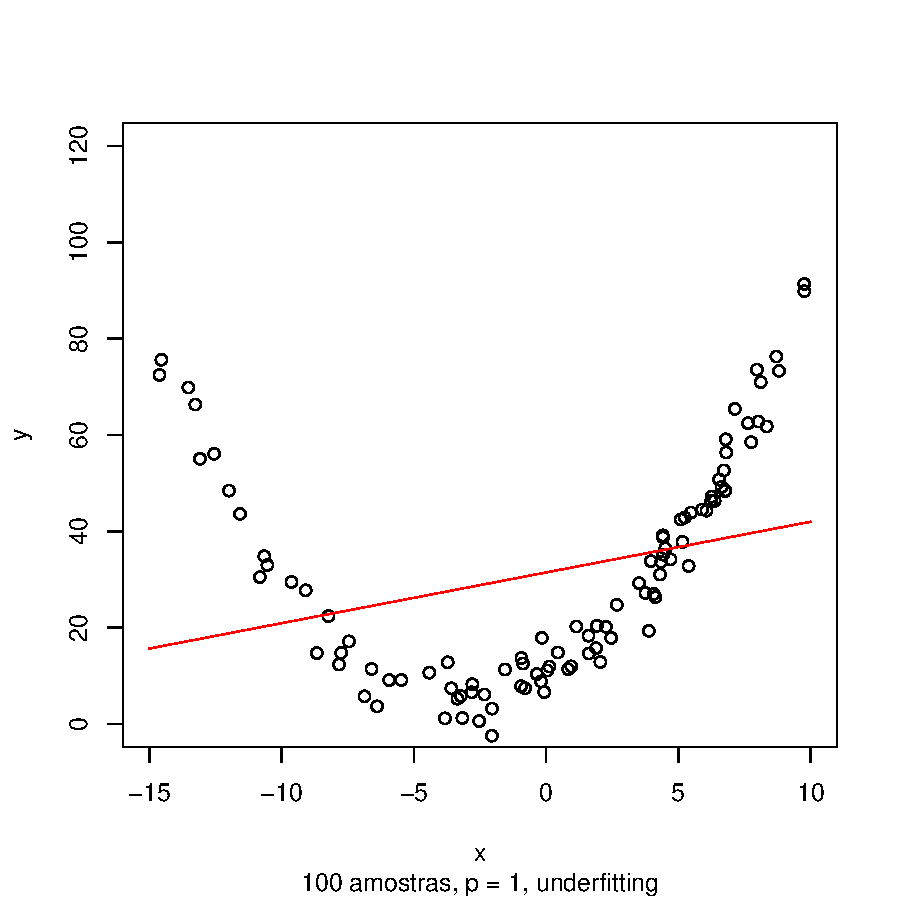
\includegraphics{aprox-011}

\subsection{p = 2}
\begin{Schunk}
\begin{Sinput}
> H <- cbind(X^2, X, 1)
> w <- pseudoinverse(H) %*% Y
> Hgrid <- cbind(xgrid^2, xgrid, 1)
> yhat <- H %*% w
> yhatgrid <- Hgrid %*% w
> plot(X, Y, type='p', xlim=c(-15,10), ylim=c(0,120), xlab='', ylab='')
> par(new=T)
> plot(xgrid, yhatgrid, type='l', xlim=c(-15,10), ylim=c(0,120),
+      col=cores[2], xlab='x', ylab='y', sub='100 amostras, p = 2, modelo balanceado')
\end{Sinput}
\end{Schunk}
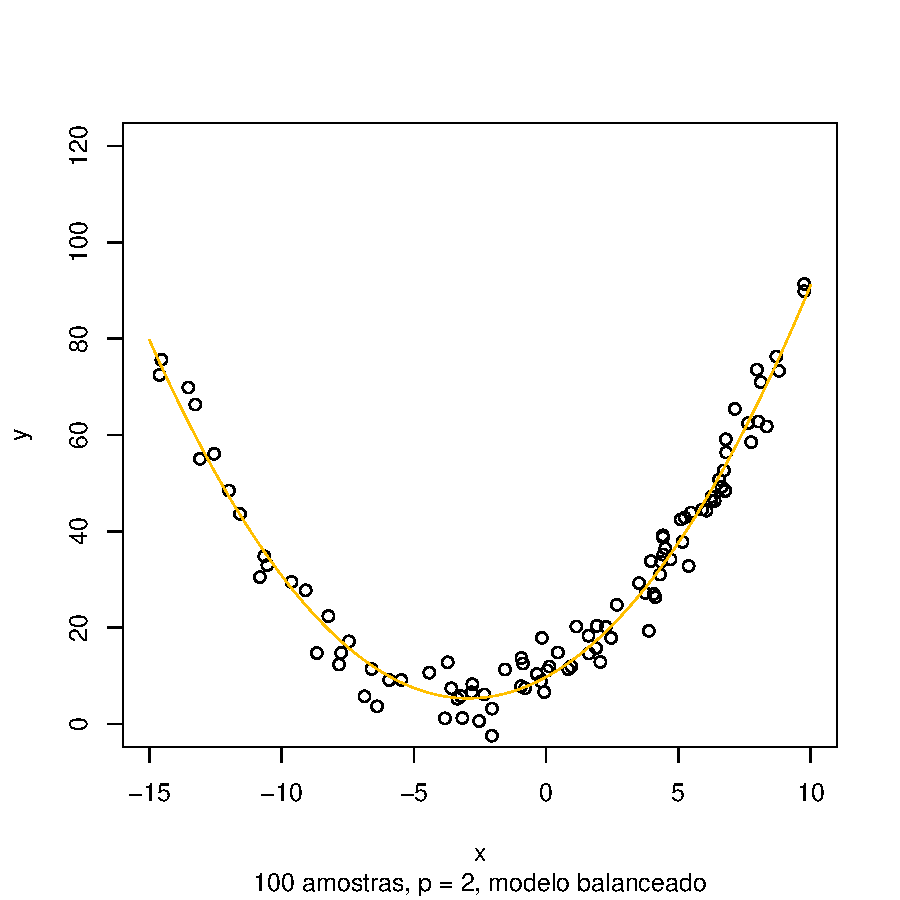
\includegraphics{aprox-012}

\subsection{p = 3}
\begin{Schunk}
\begin{Sinput}
> H <- cbind(X^3, X^2, X, 1)
> w <- pseudoinverse(H) %*% Y
> Hgrid <- cbind(xgrid^3, xgrid^2, xgrid, 1)
> yhat <- H %*% w
> yhatgrid <- Hgrid %*% w
> plot(X, Y, type='p', xlim=c(-15,10), ylim=c(0,120), xlab='', ylab='')
> par(new=T)
> plot(xgrid, yhatgrid, type='l', xlim=c(-15,10), ylim=c(0,120), 
+      col=cores[3], xlab='x', ylab='y', sub='100 amostras, p = 3, modelo balanceado')
\end{Sinput}
\end{Schunk}
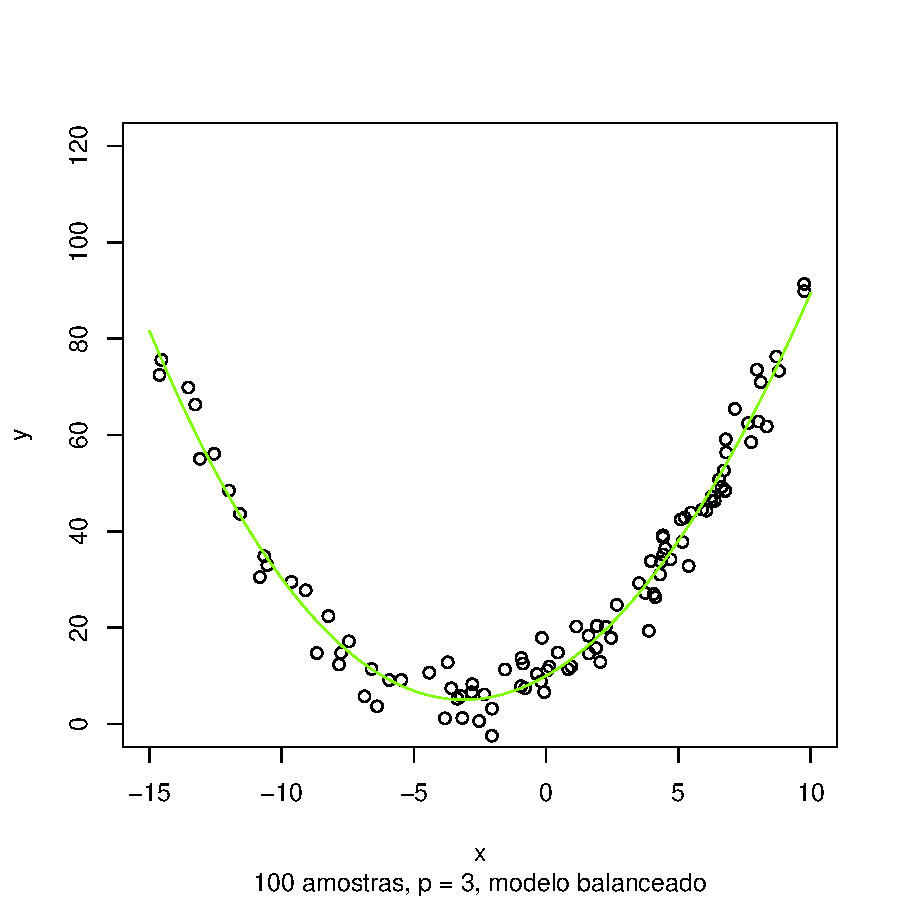
\includegraphics{aprox-013}
\subsection{p = 4}
\begin{Schunk}
\begin{Sinput}
> H <- cbind(X^4, X^3, X^2, X, 1)
> w <- pseudoinverse(H) %*% Y
> Hgrid <- cbind(xgrid^4, xgrid^3, xgrid^2, xgrid, 1)
> yhat <- H %*% w
> yhatgrid <- Hgrid %*% w
> plot(X, Y, type='p', xlim=c(-15,10), ylim=c(0,120), xlab='', ylab='')
> par(new=T)
> plot(xgrid, yhatgrid, type='l', xlim=c(-15,10), ylim=c(0,120),
+      col=cores[4], xlab='x', ylab='y', sub='100 amostras, p = 4, modelo balanceado')
\end{Sinput}
\end{Schunk}
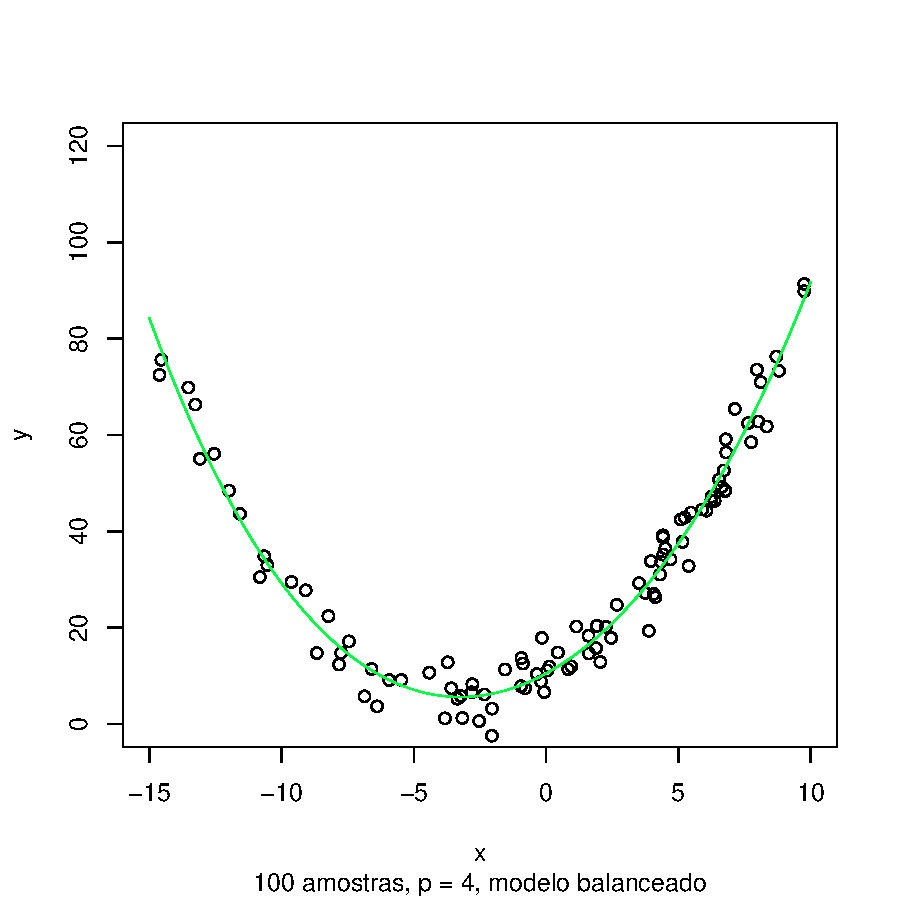
\includegraphics{aprox-014}
\subsection{p = 5}
\begin{Schunk}
\begin{Sinput}
> H <- cbind(X^5, X^4, X^3, X^2, X, 1)
> w <- pseudoinverse(H) %*% Y
> Hgrid <- cbind(xgrid^5, xgrid^4, xgrid^3, xgrid^2, xgrid, 1)
> yhat <- H %*% w
> yhatgrid <- Hgrid %*% w
> plot(X, Y, type='p', xlim=c(-15,10), ylim=c(0,120), xlab='', ylab='')
> par(new=T)
> plot(xgrid, yhatgrid, type='l', xlim=c(-15,10), ylim=c(0,120),
+      col=cores[5], xlab='x', ylab='y', sub='100 amostras, p = 5, modelo balanceado')
\end{Sinput}
\end{Schunk}
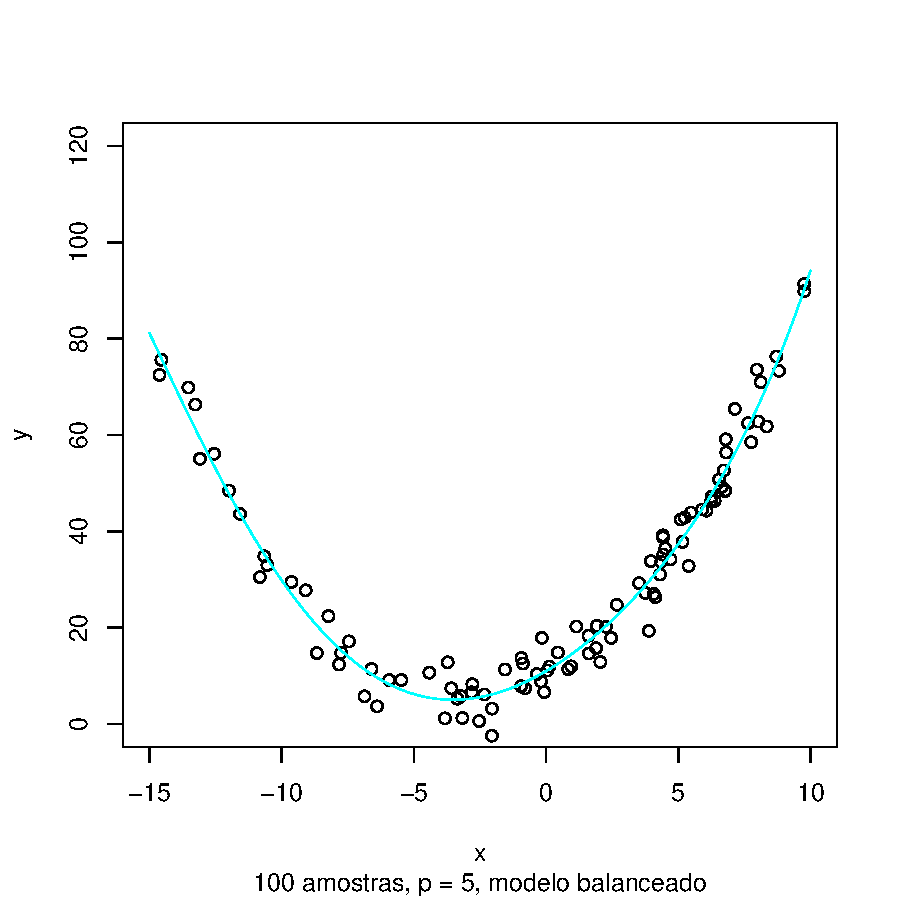
\includegraphics{aprox-015}
\subsection{p = 6}
\begin{Schunk}
\begin{Sinput}
> H <- cbind(X^6, X^5, X^4, X^3, X^2, X, 1)
> w <- pseudoinverse(H) %*% Y
> Hgrid <- cbind(xgrid^6, xgrid^5, xgrid^4, xgrid^3, xgrid^2, xgrid, 1)
> yhat <- H %*% w
> yhatgrid <- Hgrid %*% w
> plot(X, Y, type='p', xlim=c(-15,10), ylim=c(0,120), xlab='', ylab='')
> par(new=T)
> plot(xgrid, yhatgrid, type='l', xlim=c(-15,10), ylim=c(0,120),
+      col=cores[6], xlab='x', ylab='y', sub='100 amostras, p = 6, modelo balanceado')
\end{Sinput}
\end{Schunk}
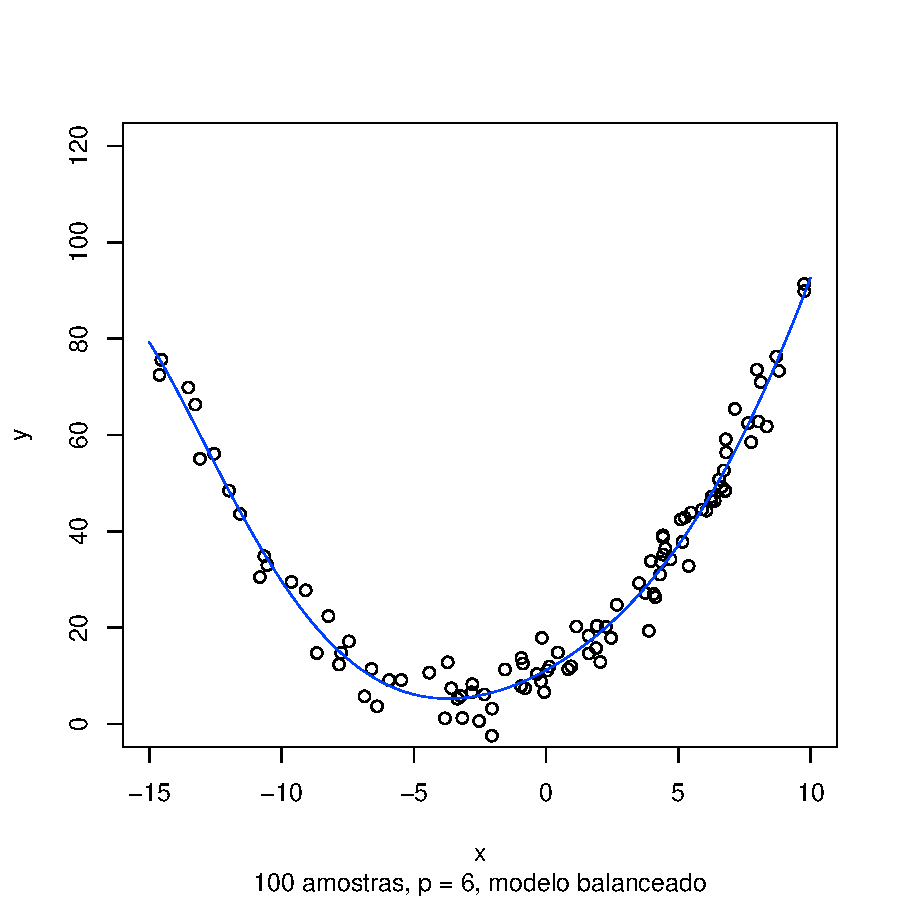
\includegraphics{aprox-016}
\subsection{p = 7}
\begin{Schunk}
\begin{Sinput}
> H <- cbind(X^7, X^6, X^5, X^4, X^3, X^2, X, 1)
> w <- pseudoinverse(H) %*% Y
> Hgrid <- cbind(xgrid^7, xgrid^6, xgrid^5, xgrid^4, xgrid^3, xgrid^2, xgrid, 1)
> yhat <- H %*% w
> yhatgrid <- Hgrid %*% w
> plot(X, Y, type='p', xlim=c(-15,10), ylim=c(0,120), xlab='', ylab='')
> par(new=T)
> plot(xgrid, yhatgrid, type='l', xlim=c(-15,10), ylim=c(0,120),
+      col=cores[7], xlab='x', ylab='y', sub='100 amostras, p = 7, overfitting')
\end{Sinput}
\end{Schunk}
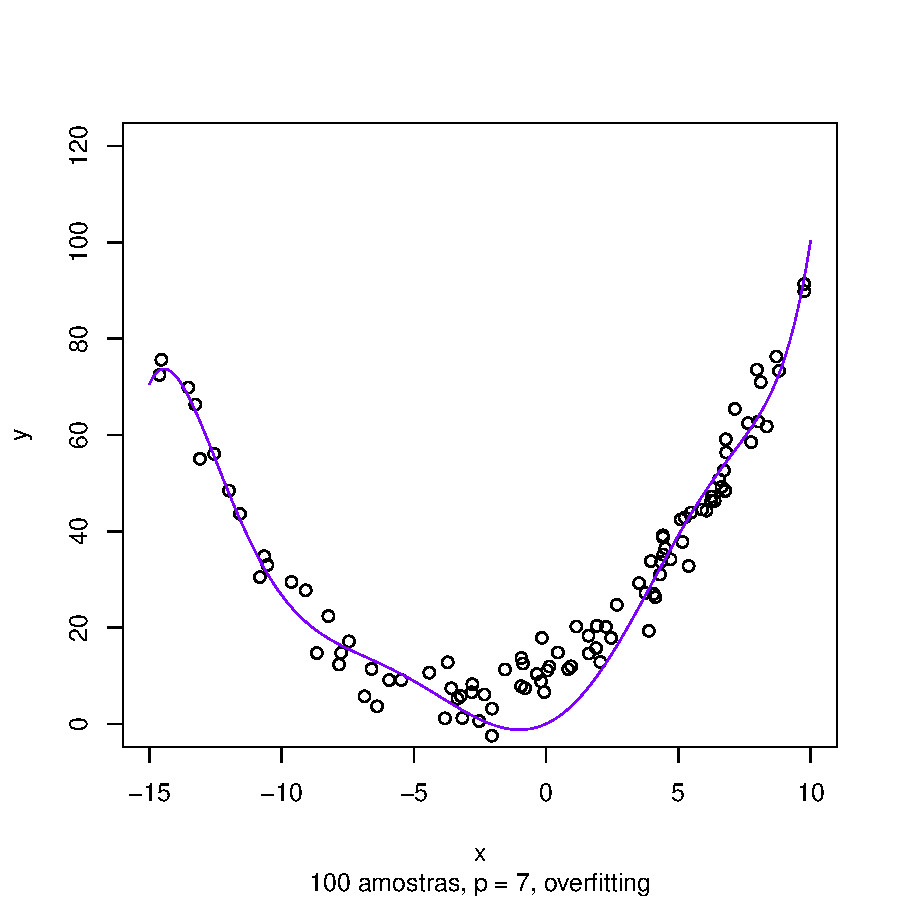
\includegraphics{aprox-017}
\subsection{p = 8}
\begin{Schunk}
\begin{Sinput}
> H <- cbind(X^8, X^7, X^6, X^5, X^4, X^3, X^2, X, 1)
> w <- pseudoinverse(H) %*% Y
> Hgrid <- cbind(xgrid^8, xgrid^7, xgrid^6, xgrid^5, xgrid^4, xgrid^3, xgrid^2, xgrid, 1)
> yhat <- H %*% w
> yhatgrid <- Hgrid %*% w
> plot(X, Y, type='p', xlim=c(-15,10), ylim=c(0,120), xlab='', ylab='')
> par(new=T)
> plot(xgrid, yhatgrid, type='l', xlim=c(-15,10), ylim=c(0,120),
+      col=cores[8], xlab='x', ylab='y', sub='100 amostras, p = 8, overfitting')
\end{Sinput}
\end{Schunk}
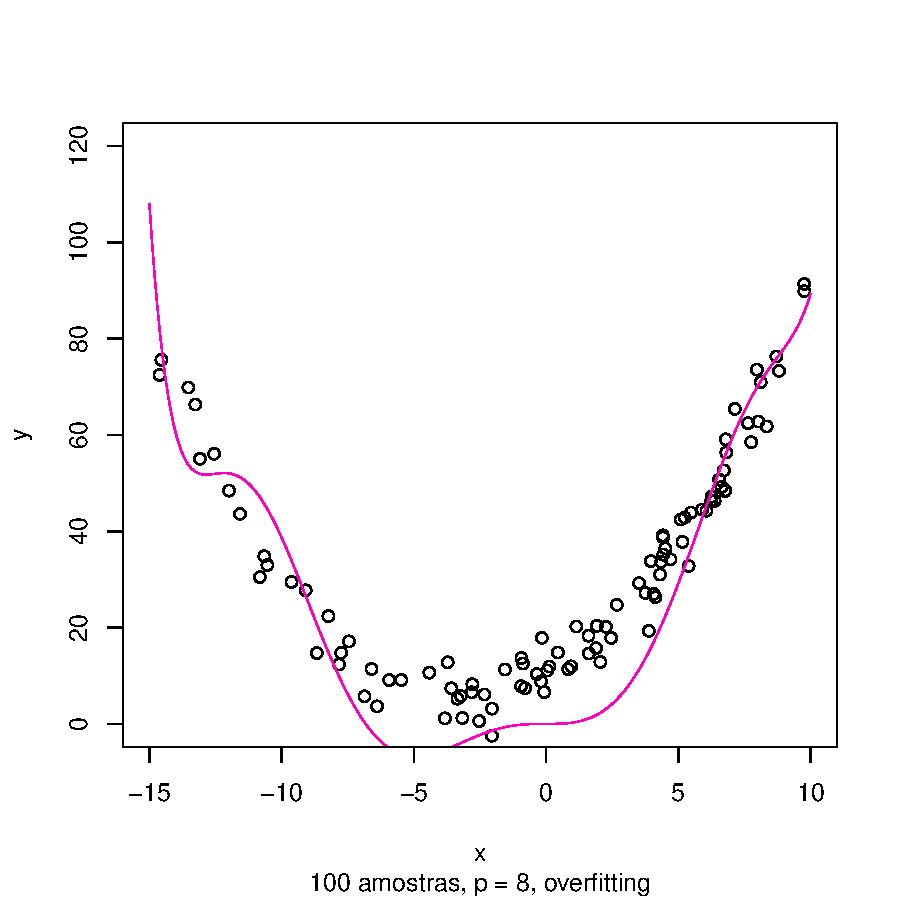
\includegraphics{aprox-018}


\end{document}
